%% GAMA-RCA manuscript -- Elsevier elsarticle (preprint layout for submission).
%% Build: latexmk -pdf main.tex   (elsarticle.cls and elsarticle-num.bst are shipped in this folder)
%% Placeholders for runs not yet finished are typeset in orange (\pending, \tbd); search for them before submission.
\documentclass[preprint,12pt]{elsarticle}

\usepackage[T1]{fontenc}
\usepackage[utf8]{inputenc}
\usepackage{lmodern}

\usepackage{amsmath,amssymb,amsfonts}
\usepackage{bm}
\usepackage{graphicx}
\usepackage{rotating}
\usepackage{float}
\usepackage[section]{placeins}
\usepackage{booktabs}
\usepackage{multirow}
\usepackage{array}
\usepackage{tabularx}
\usepackage{threeparttable}
\usepackage[table]{xcolor}
\usepackage{siunitx}
\usepackage{algorithm}
\usepackage{algpseudocode}
\usepackage{enumitem}
\usepackage{lineno}
\usepackage[hidelinks]{hyperref}
\usepackage[capitalise,nameinlink]{cleveref}

\sisetup{detect-all, group-separator={,}, group-minimum-digits=4}
\setlist{nosep, leftmargin=*}
\definecolor{pend}{HTML}{C2410C}
\newcommand{\pending}[1]{\textcolor{pend}{\textbf{[Pending: #1]}}}
\newcommand{\tbd}{\textcolor{pend}{\textbf{XX}}}
\newcommand{\gama}{GAMA-RCA}
\newcommand{\core}{GAMA}
\newcommand{\Mod}[1]{\textsf{M#1}}
\newcommand{\sig}[1]{\nolinkurl{#1}}
\makeatletter\g@addto@macro{\UrlBreaks}{\do\_}\makeatother
\DeclareMathOperator*{\argmax}{arg\,max}
\DeclareMathOperator{\median}{med}
\DeclareMathOperator{\mad}{MAD}
\renewcommand{\arraystretch}{1.12}

\journal{(target journal -- to be decided)}

\begin{document}

\begin{frontmatter}

\title{\gama: Graph-aware, Multimodal, Abductive Root Cause Analysis for Microservices with a Computed Belief and a Bounded Language Model}

%% Authors and affiliations as in the earlier manuscript -- to be confirmed by the authors.
\author[ugm]{Achmad Solaeman\corref{cor1}}
\ead{achmad.solaeman@ugm.ac.id}
\author[ugm]{Nur Rohman Rosyid}
\author[ugm]{Ardhi Wicaksono}
\author[ugm]{Prima Asmara Sejati}
\author[mpki]{Hamzah}
\cortext[cor1]{Corresponding author.}
\affiliation[ugm]{organization={Department of Electrical Engineering and Informatics, Vocational College, Universitas Gadjah Mada},
            city={Yogyakarta}, country={Indonesia}}
\affiliation[mpki]{organization={PT Media Pangan Kreatif Indonesia}, country={Indonesia}}

\begin{abstract}
Root cause analysis (RCA) of microservice failures must name the faulty component, its fault mechanism and the propagation path
from metrics, logs, traces and events. Agents built on large language models (LLMs) reason over this telemetry at a cost of up to
millions of tokens per incident, with conclusions that are hard to audit. We present \gama{}, a label-free method in which the
diagnosis is \emph{computed}. Every signal is scored against the incident's own history and its peers and calibrated on
pseudo-windows cut from that history; the observations update a Bayesian belief over (entity, fault type) hypotheses with
fingerprint-based likelihoods, topology explain-away, a per-incident propagation strength estimated by expectation--maximisation,
and temporal precedence. A two-stage decision names the root entity and its type, and a deterministic chain cites the evidence of
every step. An optional, bounded LLM may read log text, choose a type from the statistical shortlist and narrate the chain. On the
103 cases of RCA100, the statistical core reaches a Final score of 62.9 [95\% CI 57.4, 68.5] on a CPU, 20.2 points above an LLM that
decides from the same evidence ($p=2.8\times10^{-10}$). In a pre-registered study, the bounded LLM lowers the score by 3.7
(Qwen2.5-7B) and 3.5 points (gpt-oss-120b): scale does not improve the decision, but it improves the explanation, raising the
narrator's evidence-checkpoint rate from 0.107 to 0.284, close to the computed chain (0.307). \pending{zero-shot AIOps2025 result.}
\end{abstract}

\begin{highlights}
\item The diagnosis is a computed posterior over (entity, fault type), not text written by a language model.
\item Every signal is calibrated against the incident's own history and peers; no labels and no training are used.
\item The statistical core reaches 62.9 Final on RCA100 on a CPU, 20 points above an LLM given the same evidence.
\item A larger LLM does not decide better (both backbones lower the score), but it explains far better.
\item All evaluation runs, hypotheses and amendments were pre-registered and are released with every prompt and output.
\end{highlights}

\begin{keyword}
root cause analysis \sep microservices \sep AIOps \sep Bayesian inference \sep observability \sep large language models
\sep explainability
\end{keyword}

\end{frontmatter}
\linenumbers

\section{Introduction}\label{sec:intro}

A microservice application is a graph of independently deployed services that call each other over the network and share
hosts, caches and databases. When one component fails, the failure crosses component boundaries: an exhausted CPU on a node slows
every service it hosts, a failing payment service returns errors to the checkout service that calls it, and the operator sees
alerts far from the cause \citep{avizienis2004taxonomy,soldani2022anomaly}. Root cause analysis (RCA) must therefore answer three
questions from the incident's telemetry---metrics, logs, traces, Kubernetes events and the service topology: \emph{which} entity is
the root cause, \emph{what} fault mechanism acts there, and \emph{how} the fault propagated to the symptoms
\citep{zhang2025survey,fu2025survey}. Recent benchmarks score all three. RCA100 \citep{cai2026benchmark} grades entity localisation,
fault identification over 28 fault types and the reasoning process along a typed causal chain with numeric evidence checkpoints.

Two families of methods address the task. Statistical and causal methods rank candidate components from metric changes, trace
structure or learned causal graphs \citep{wu2020microrca,ikram2022rcd,pham2024baro,li2022circa,yu2023nezha,zheng2024mulan}. They are
cheap and reproducible, but they usually return a ranked list of components without a fault type or an explanation. Agents built on
large language models (LLMs) read the telemetry through tools and write a diagnosis in natural language
\citep{chen2024rcacopilot,wang2024rcagent,xu2025openrca,pei2025flowofaction,zhang2024mabc}. They produce types and explanations,
but a trajectory-level study of such agents finds systematic reasoning failures---untested baselines, ignored timing, reversed
caller / callee semantics, anchoring on the first hypothesis \citep{lu2026beyond,riddell2026stalled}---and the strongest agents
consume on the order of $10^6$ tokens per incident \citep{lu2026beyond,luo2026pos}. Agents that maintain an explicit belief state
\citep{luo2026pos,luo2026graphofstates} still ask the LLM to \emph{write} that belief.

This paper takes the opposite position: the belief over root causes can be \emph{computed} from calibrated evidence, and the
language model, if used at all, should be bounded to the parts that need language. We present \gama{} (Graph-aware, Multimodal,
Abductive RCA). Every continuous signal of every entity is scored against the incident's own history and its peers, and the score
is turned into a p-value by an empirical null cut from that history (pseudo-windows); events, status codes, failing spans and log
text become categorical observations. A Bayesian model over (entity, fault type) hypotheses scores these observations with
fingerprints that state, for each fault type, which signals are key, supporting, possible consequences or contradictions. Symptoms
that a hypothesis can explain along the topology are explained away; the propagation strength is a per-incident nuisance parameter
estimated by expectation--maximisation; and a root may not start after the symptoms it explains. The decision is two-stage (entity,
then type), and the causal chain is computed along the topology, citing the window values of every step. An optional LLM may read
log text chosen by expected information gain, choose a type from the statistical shortlist with a verbatim quote, and narrate the
chain.

We evaluate \gama{} on the 103 cases of RCA100 under a pre-registered protocol (hypotheses, statistics and every amendment
recorded before the corresponding run) and release every prompt and output. The results support three statements. First, the
statistical core alone reaches a Final score of 62.9, on a CPU and without labels, 20.2 points above an LLM that decides from the
same calibrated evidence and 44.1 points above an LLM that reads the alert only. Second, the bounded LLM lowers the decision score
by 3.7 (Qwen2.5-7B) and 3.5 points (gpt-oss-120b): when the telemetry cannot separate two fault types, the LLM tends to pick the
more specific one and is more often wrong than right. Third, scale improves the \emph{explanation}: the narrator of the larger model
hits 2.7 times as many step-anchored evidence checkpoints as the 7B narrator, close to the computed chain. We then transfer the
method zero-shot to AIOps2025 \citep{cai2026benchmark}, a different system with different fault types, changing only
dataset knowledge (an adapter and a fingerprint table written from the published fault definitions).

\paragraph{Contributions}
\begin{enumerate}
\item \textbf{A computed abductive belief for RCA.} A label-free likelihood model over (entity, fault type) hypotheses with
fingerprint roles, topology explain-away, per-incident propagation strength (EM) and temporal precedence (\cref{sec:method}).
\item \textbf{Calibrated multimodal evidence.} Shift scores against the incident's own history and peers, calibrated on
pseudo-windows, together with trace-origin attribution, direction-aware load explain-away, mechanism-naming text and cross-modal
corroboration as separable modules (\Mod{1}--\Mod{6}).
\item \textbf{A pre-registered study of what an LLM adds.} Seven arms on the same 103 cases, from an LLM that sees only the alert
to the computed belief alone, two backbones (7B local, 120B through an API) and hypotheses fixed in advance
(\cref{sec:setup,sec:results}): the LLM does not improve the decision at either scale, while scale improves the explanation.
\item \textbf{A zero-shot transfer protocol} to an unseen system, pre-registered with an implementation audit, and an open
implementation with equivalence and synthetic tests (\cref{sec:aiops}).
\end{enumerate}

The paper is organised as follows. \Cref{sec:related} reviews related work, \cref{sec:problem} states the problem and the metrics,
\cref{sec:method} describes the method, \cref{sec:setup} the experimental protocol, \cref{sec:results} the results,
\cref{sec:discussion} discusses implications and threats to validity, and \cref{sec:conclusion} concludes.

\section{Related work}\label{sec:related}

\paragraph{Statistical and causal RCA}
Graph-based methods propagate anomaly scores over the call graph \citep{wu2020microrca,lin2018microscope}; MicroHECL distinguishes
performance, reliability and traffic anomalies by their direction of propagation \citep{liu2021microhecl}. Causal methods learn a
graph from metric time series or recognise the intervention that a fault represents \citep{ikram2022rcd,li2022circa,meng2020microcause}.
BARO detects multivariate change points with a Bayesian online model and ranks the changed services \citep{pham2024baro};
$\epsilon$-Diagnosis tests small windows against history \citep{shan2019epsilon}. Trace-based methods locate the deepest failing or
slowest span \citep{li2021tracerca,yu2021microrank,guo2020graphtrace}. Multimodal methods fuse metrics, logs and traces into shared
representations or event graphs, often with training \citep{zhang2023diagfusion,lee2023eadro,yu2023nezha,zheng2024mulan}. These
methods share our preference for computation over generation, but most output a ranking of components; fault types and an
evidence-cited causal chain are outside their scope, and the evidence from different modalities is usually fused before any
reasoning about mechanisms. \gama{} keeps the statistical tests of this line of work but places them in a likelihood over typed
hypotheses, so that the same model names the entity, the mechanism and the evidence.

\paragraph{Probabilistic diagnosis}
Explaining away \citep{pearl1988probabilistic} and noisy propagation over dependency graphs \citep{bahl2007sherlock} are the
classical foundations of our belief model; active probing with information gain \citep{rish2005adaptive,lindley1956information}
motivates the text sensor. Calibration of test scores against an empirical null \citep{efron2004null} and conformal calibration
\citep{vovk2005conformal} motivate our pseudo-window p-values. Compared with these works, \gama{} instantiates the hypothesis space
with fault \emph{types} from a benchmark taxonomy, derives likelihoods from fingerprint roles instead of training, and estimates the
propagation strength per incident.

\paragraph{LLM-based RCA}
RCACopilot predicts incident categories from collected diagnostic information \citep{chen2024rcacopilot}; RCAgent and ReAct-style
agents call tools in an open loop \citep{wang2024rcagent,yao2023react,roy2024exploring}; Flow-of-Action and mABC organise several
agents around procedures or votes \citep{pei2025flowofaction,zhang2024mabc}; GALA refines a statistical ranking with agentic
re-ranking \citep{tian2025gala}. OpenRCA, RCAEval, AIOpsLab and RCA100 turn the task into benchmarks
\citep{xu2025openrca,pham2025rcaeval,chen2025aiopslab,cai2026benchmark}; OpenRCA~2.0 adds causal process supervision
\citep{fang2026openrca2}. Lu et al.\ \citep{lu2026beyond} analyse agent trajectories on RCA100 and AIOps2025 and catalogue omission,
misreading and generation failures; Riddell et al.\ \citep{riddell2026stalled} report stalled and biased reasoning. Closest to our
bounded LLM are the combination of an LLM with a small classifier \citep{han2024oneshot}, confidence estimation for root causing
\citep{zhang2024lmpace} and grounding / verification of generated claims \citep{venktesh2025verify,gao2023alce}.

\paragraph{Belief states and abduction with LLMs}
Long-horizon agents that maintain an explicit belief state, or a graph of hypothesis states, improve over memory-only agents on
abductive tasks including RCA100 \citep{luo2026pos,luo2026graphofstates}; planning under uncertainty with LLM-generated hypotheses
follows the POMDP view \citep{kaelbling1998pomdp,tang2026trupomdp}. In these systems the LLM writes and updates the belief. In
\gama{} the belief is a posterior computed from calibrated likelihoods; the LLM can only contribute a likelihood term (sensor) or a
choice among statistically ranked options (typing).

\Cref{tab:positioning} summarises the positioning, and \cref{tab:failuremodes} (\ref{app:failuremodes}) maps the failure modes
catalogued by Lu et al.\ \citep{lu2026beyond} to the mechanism of \gama{} that rules each out by construction.

\begin{table}[!htbp]
\centering
\caption{Positioning of \gama{} among RCA approaches.}\label{tab:positioning}
\small
\begin{tabularx}{\textwidth}{@{}l>{\raggedright\arraybackslash}X>{\raggedright\arraybackslash}X>{\raggedright\arraybackslash}X l@{}}
\toprule
Approach & Decision made by & Output & Evidence calibration & Labels \\
\midrule
Statistical / causal \citep{wu2020microrca,ikram2022rcd,pham2024baro} & scores / causal graph & ranked components & per method & no \\
Multimodal learned \citep{lee2023eadro,zhang2023diagfusion} & trained model & component, type & learned & yes \\
LLM agents \citep{wang2024rcagent,xu2025openrca,pei2025flowofaction} & LLM & free text, chain & none (LLM reads raw data) & no \\
Belief-state agents \citep{luo2026pos} & LLM-written belief & entity, type, chain & none & no \\
\textbf{\gama{} (this work)} & \textbf{computed posterior} & \textbf{entity, type, cited chain} & \textbf{history, peers, pseudo-windows} & \textbf{no} \\
\bottomrule
\end{tabularx}
\end{table}

\section{Problem statement and evaluation metrics}\label{sec:problem}

\paragraph{Incident}
An incident (case) consists of an alert window $W=[w_0,w_1]$ with an alert text and, when available, the alerted service and
operation; a topology graph $G$ whose nodes are services, operations, pods and hosts (nodes) and whose edges are \emph{calls} and
\emph{hosting} relations; and the telemetry of the window and of the time before it: metric series per entity, log lines, spans of
distributed traces and Kubernetes events. No label is available at diagnosis time.

\paragraph{Output}
A diagnosis is a triple $(e^\ast,\tau^\ast,C)$: the root-cause entity $e^\ast$ (a service or a node), its fault type $\tau^\ast$ from a
fixed taxonomy $\mathcal{T}$, and a causal chain $C$ of steps \emph{cause} $\rightarrow$ \emph{propagation} $\rightarrow$
\emph{impact}, each naming an entity and the evidence (signal and value) that supports it. Following the dependability vocabulary
\citep{avizienis2004taxonomy}, the root cause is the component where the fault is activated; the chain records how the resulting
errors and load cross component boundaries to the alerted operation.

\paragraph{Metrics}
We use the three pillars of the RCA100 protocol \citep{cai2026benchmark}. \emph{Entity localisation} (EL) is 1 for the true entity
and $0.5^d$ for an entity at topological distance $d$. \emph{Fault identification} (FI) is 1 for the exact type and 0 otherwise.
The \emph{reasoning process} (RP) is the mean of (i) the share of ground-truth chain nodes named by the predicted chain and (ii) the
share of ground-truth evidence checkpoints satisfied, where a checkpoint is a signal with a numeric constraint (e.g.\
\texttt{error\_count} $\geq 8829$) that the cited evidence must meet. The Final score is
\begin{equation}
\text{Final} = 0.4\,\text{EL} + 0.3\,\text{FI} + 0.3\,\text{RP},
\end{equation}
reported on a 0--100 scale. In the headline RP the checkpoints are searched in the evidence the system retrieved; this rewards
systems that return evidence items and gives zero to a chain written by an LLM without them. We therefore also report a
\emph{step-anchored} variant (Final$_\text{step}$), in which a checkpoint counts only if the chain step that names the
checkpoint's target entity cites a value meeting the constraint. An official scoring script was not part of the RCA100 release we used;
our scorer is a re-implementation of the published protocol and is released with the code. We also count the cases with the exact
entity, the exact type and both (joint).

\section{Method}\label{sec:method}

\Cref{fig:arch} shows the pipeline. Three principles guided every design decision.
\textbf{P1, calibrate, do not threshold:} every observation is scored against the incident's own history and peers, and
likelihoods use rates rather than cut-offs.
\textbf{P2, causes precede and propagate directionally:} errors travel up the call graph to callers and load travels down to
callees; a symptom the root can explain is not evidence against it, and load that came from upstream is not evidence for a
downstream root.
\textbf{P3, the LLM reads text and chooses among ranked options:} the decision and its evidence are computed.
The method has a core (stages 1--3 and the chain) and seven switchable modules: \Mod{1}--\Mod{6} form the statistical core
(\core{}), and \Mod{7} is the bounded LLM. All constants are listed in \cref{tab:constants} (\ref{app:constants}); none was fitted
to labels.

\begin{sidewaysfigure}
\centering
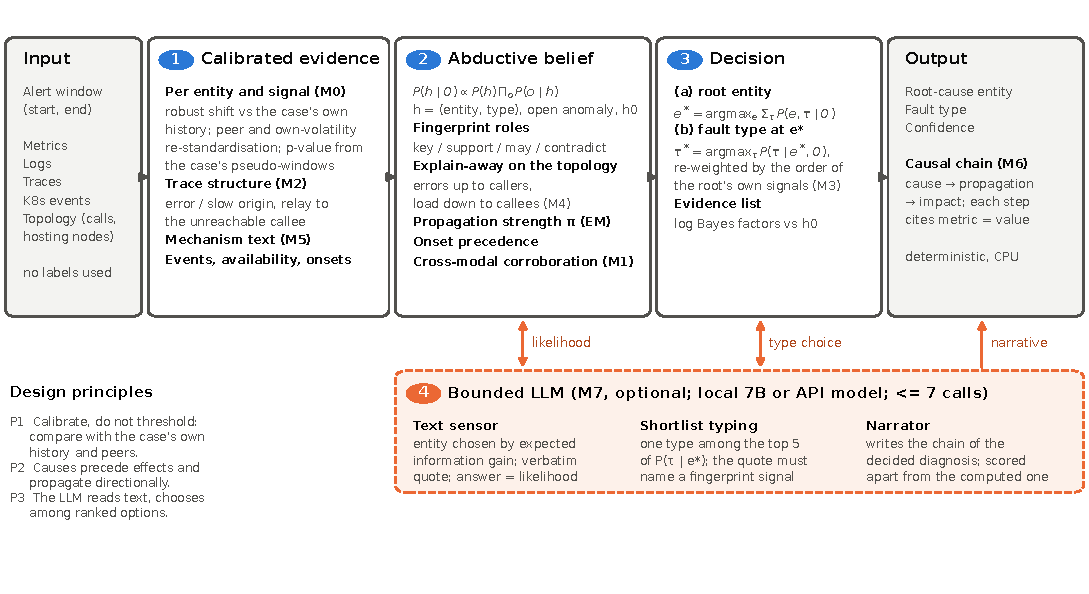
\includegraphics[width=\textheight]{figs/fig1_architecture.pdf}
\caption{\gama{}. Stage 1 turns telemetry into calibrated binary observations; stage 2 computes a posterior over (entity, fault
type) hypotheses; stage 3 decides the root entity and then its type; the chain (\Mod{6}) cites window values along the topology
path. The bounded LLM (stage 4, optional) contributes a likelihood term (sensor), a choice among the statistical shortlist (typing)
and a narrative that is scored separately.}\label{fig:arch}
\end{sidewaysfigure}

\subsection{Stage 1: calibrated evidence}\label{sec:evidence}

\paragraph{Signals}
Metric series are mapped to signal families by their names (CPU, memory, garbage collection, threads, disk, throttling, request
count, latency, errors, restarts, replicas / availability); configuration constants (limits, initial sizes) are excluded. For a
service the signals are, for instance, \sig{svc_cpu_rise}, \sig{svc_latency_rise} or \sig{svc_request_drop}; for a node
\sig{node_cpu_rise}, \sig{node_mem_rise}, \sig{node_disk_rise} and \sig{node_ready_drop}. Each signal has a direction
$d\in\{+1,-1\}$ (rise or drop).

\paragraph{Robust shift}
Let $x$ be a series of entity $e$ and $[a,b)$ a tested window of length $L=b-a$. Its history is $\mathcal{H}=[a-BL,a)$ with $B=4$.
The directional robust shift is
\begin{equation}\label{eq:shift}
\begin{aligned}
z &= d\cdot\frac{\median_{t\in[a,b)} x_t-\median_{t\in\mathcal{H}} x_t}{\sigma_{\mathcal{H}}},\\
\sigma_{\mathcal{H}} &= \max\!\big(1.4826\,\mad_{\mathcal{H}}(x),\;0.05\,|\median_{\mathcal{H}} x|,\;\epsilon\big),
\end{aligned}
\end{equation}
computed only when the history covers at least 80\% of its expected samples and the window at least half of them. Error counts are
summed in 30\,s bins (zero-filled) with a scale floor of one event per bin. The score of a signal is the largest $z$ over the
entity's series of that family.

\paragraph{Pseudo-windows and calibration}
A shift score is not a probability: series drift and are autocorrelated, so the window and its history are not exchangeable, and a
plain rank test flagged about 30\% of fault-free windows in our development runs. We therefore compute the same score on $K=5$
pseudo-windows $W_j=[w_0-jL,\,w_0-(j-1)L)$ cut from the incident's own pre-alert data, each against its own history. Two
re-standardisations are applied identically to real and pseudo scores. \emph{Own volatility}: each entity's score is re-centred and
re-scaled by the median and MAD of its pseudo scores (leave-one-out for the pseudo-windows, floor 1), so a chronically noisy entity
does not outrank one that changed only now. \emph{Peers}: in every window the score is re-standardised against the scores of the
other entities of the same kind (at least three peers, floor 1), which rejects a load step or a drift that moves all of them. The
calibrated p-value of the real window is the conformal rank of its score among the pseudo scores of all entities of the same kind
and signal in the incident \citep{efron2004null,vovk2005conformal},
\begin{equation}\label{eq:pvalue}
p = \frac{1+\#\{z'\in\mathcal{N}_{k,s}: z'\geq z\}}{|\mathcal{N}_{k,s}|+1},
\end{equation}
pooled over the entity kind when fewer than 20 pseudo scores exist. The signal \emph{holds} when $p\leq\alpha=0.05$. The
\emph{onset} of a holding signal is the first sample whose shift against a history ending one window earlier reaches 3 for two
consecutive samples.

\paragraph{Categorical observations}
Kubernetes events (OOM kill, crash loop, failed probe, scheduling failure, scale-down, restart, eviction, node not ready) count only
when their increments inside the window exceed their own long-run rate (Poisson test). Availability below the desired replica count
is a state. Failing spans contribute their HTTP / gRPC status class and the mechanism named by their message (null pointer, rate
limit, DNS, connection refused, timeout, Redis, out of memory, GC, thread pool, queue, load balancer, network policy, SQL, cache);
failing or slow dependency spans (database, cache, queue) are separate signals. The background rate of a categorical observation is
the share of entities of the same level showing it in the incident, shrunk towards $\alpha$ with a Beta prior worth ten
pseudo-entities. Each incident yields on the order of $10^3$ binary observations
$o=(e,s,\textit{holds},\textit{onset})$.

\subsection{Stage 2: abductive belief}\label{sec:belief}

\paragraph{Hypotheses}
For every service $e$ and fault type $\tau$ of service level, and every node and type of node level, $h=(e,\tau)$ is a hypothesis;
each entity also has an open hypothesis ``anomaly of unspecified type'', and $h_0$ denotes no fault. A hypothesis is \emph{testable}
only if at least one of its key signals was computed. The posterior is
\begin{equation}
\Pr(h\mid O)\;\propto\;\Pr(h)\prod_{o\in O}\Pr(o\mid h),
\end{equation}
with equal prior mass per entity, split among its hypotheses (the two fallback types of the taxonomy, \emph{httpError5xx} and
\emph{codeDefect}, at half weight), and $\Pr(h_0)=0.1$.

\paragraph{Fingerprint roles}
For each type, a fingerprint written from the taxonomy definitions assigns roles to signals: \emph{key} (at least one must hold),
\emph{support}, \emph{may} (a possible consequence, whose absence is uninformative) and \emph{contradiction}. For example,
\emph{cpuFullLoad} has the key \sig{svc_cpu_rise}, the support \sig{svc_latency_rise} and the contradiction
\sig{svc_request_rise} (a CPU rise caused by more traffic is a traffic fault). For an observation at the hypothesised root,
\begin{equation}\label{eq:roles}
\Pr(o\text{ holds}\mid h)=\begin{cases}
q_h & \text{key},\quad q_h=1-(1-\theta_K)^{1/n_h}\\
\theta_U & \text{support or may}\\
\alpha_C & \text{contradiction}\\
\beta_s & \text{otherwise (background)},
\end{cases}
\end{equation}
where $n_h$ is the number of testable keys, so that the probability that some key holds is $\theta_K$. Symptoms expected at any root
(latency, errors, failing spans) have probability $\max(\theta_P,\beta_s)$, and the absence of a \emph{may} signal leaves the
likelihood at its $h_0$ value.

\paragraph{Explaining away along the topology}
Let $\mathrm{Expl}(e)$ be the entities whose fault can show as a symptom at $e$: the downstream closure of $e$ in the call graph and
the nodes hosting $e$ or any of them. A symptom at $e\neq e_h$ with $e_h\in\mathrm{Expl}(e)$ is a \emph{propagated} observation:
it holds with probability $\pi$, the per-incident propagation strength. A node CPU rise is explained by a root whose fault loads its
host. All other observations away from the root keep their background rates, so a hypothesis that explains many symptoms is not
rewarded for symptoms that do not occur: a wide hypothesis pays $\log(1-\pi)$ for every reachable entity that stays quiet.

\paragraph{Propagation strength by EM}
Write $\log\Pr(O\mid h)=\ell_0(h)+n^{+}(h)\log\pi+n^{-}(h)\log(1-\pi)$, where $n^{\pm}(h)$ count the propagated symptoms that hold or
are absent. Expectation--maximisation \citep{dempster1977em} alternates the posterior $w_h\propto\Pr(h)\,\Pr(O\mid h)$ and
\begin{equation}
\pi\leftarrow\frac{\sum_h w_h\,n^{+}(h)}{\sum_h w_h\,\big(n^{+}(h)+n^{-}(h)\big)},
\end{equation}
clipped to $[0.06,0.95]$, until $\pi$ changes by less than $10^{-4}$ (at most 30 iterations).

\paragraph{Temporal precedence}
A root does not start after what it causes. For $h$ with root $e_h$ whose onset $t_{e_h}$ is measured, every explained entity with an
onset $t_e$ contributes $\log(\theta_T/0.5)$ if $t_e\geq t_{e_h}-60$\,s and $\log((1-\theta_T)/0.5)$ otherwise; a root without a
measured onset is neutral. Onsets of load explained from upstream (\Mod{4}) are ignored.

\subsection{Modules}\label{sec:modules}

\paragraph{\Mod{1} Cross-modal corroboration}
A real fault tends to leave aligned evidence in several modalities, whereas the noise of a volatile entity tends to stay in one
\citep{zhang2023diagfusion,cai2026benchmark}. Let $k(h)$ be the number of modalities (metrics, logs, traces, events) among the
holding key, support or may signals at the root. If $k(h)\geq2$ the hypothesis gains $\log(\theta_M/\beta_M)$, where $\beta_M$ is the
share of the incident's specific hypotheses with such corroboration, shrunk to a floor of 0.1; absence is uninformative.

\paragraph{\Mod{2} Trace-origin attribution}
In every failing trace the error origins are the deepest failing spans, none of whose children fails; a service is an error origin
when it originates at least 30\% of the failing traces and at least ten of them. In every trace the service with the largest self
time (span duration minus the time covered by its children) is where the time is spent; a service is a slow origin when its share
among the slowest 10\% of the traces of a root operation exceeds its share among the others by at least 0.2, in at least five
traces. A failing client span that names an unreachable callee relays the origin to that callee, past
the reporting caller \citep{li2021tracerca}. An origin is own evidence of its entity (and of a node that hosts at least two origin
services), and the messages and codes of origin spans enter as categorical observations.

\paragraph{\Mod{3} Mechanism typing}
The type stage uses three rules. A node CPU rise is explained by any root whose own CPU rises. Error origins are expected only by
types whose fingerprint names an error signal. Within the root, the cause moves before its consequences: for a type whose key is a
resource signal (CPU, memory, GC, threads), $\theta_T$ applies if that key is among the earliest-onset resource signals of the root,
$0.5$ if it holds without a measured onset and $1-\theta_T$ otherwise. This term re-weights the types of the decided root; it
does not move the root. Exact ties are broken general-before-special by the fingerprint order.

\paragraph{\Mod{4} Direction-aware load explain-away}
A request-count rise at a callee whose caller's requests rise too is load that came from upstream \citep{liu2021microhecl}: its
request, latency and CPU rises, and the CPU rise of the nodes hosting it, receive the background $\theta_P$ for every hypothesis.

\paragraph{\Mod{5} Mechanism-naming text}
Span exception text and gRPC status codes are read as mechanism evidence. A log text family becomes an observation only if it is
new in the window (Poisson test against the same length of history) and names a mechanism; symptom text (``timeout'',
``refused'') is excluded, because almost any fault produces it.

\paragraph{\Mod{6} Evidence-cited chain}
The chain follows a shortest call path from the decided root to the alerted service (for a node root, from the hosted service
closest to it) and ends at the alerted operation. Each step cites up to four window values of its own target (golden signals:
requests, errors, latency for services; CPU, memory, disk for nodes \citep{beyer2016sre}); the cause step first cites the readings
behind the root's holding evidence.

\subsection{Stage 3: decision}\label{sec:decision}
The decision is two-stage. The root entity maximises the marginal posterior,
$e^\ast=\argmax_{e}\sum_{\tau}\Pr(e,\tau\mid O)$ ($h_0$ excluded, since an alert fired), and the type maximises the conditional
posterior at that entity, $\tau^\ast=\argmax_{\tau}\Pr(\tau\mid e^\ast,O)$, after the \Mod{3} re-weighting. When only the open
anomaly is testable at $e^\ast$, the type with the strongest key evidence of its level is returned. The evidence list contains the
observations whose log Bayes factor for the decided hypothesis against $h_0$ exceeds 0.5 in absolute value; it is the material the
chain and the LLM cite. \Cref{alg:gama} summarises stages 1--3.

\begin{algorithm}[!htbp]
\caption{\core{} on one incident (no labels, no training)}\label{alg:gama}
\small
\begin{algorithmic}[1]
\Require window $[w_0,w_1]$, topology $G$, telemetry, fingerprints $F$, modules $\mathcal{M}\subseteq\{\Mod{1},\dots,\Mod{6}\}$
\State $O\gets\emptyset$
\ForAll{entities $e$, signals $s$}
  \State $z_0,\dots,z_K\gets$ shifts of the real window and the $K$ pseudo-windows (\cref{eq:shift})
  \State re-standardise by own volatility and by peers; $p\gets$ conformal rank (\cref{eq:pvalue}); add $(e,s,p\le\alpha,\text{onset})$ to $O$
\EndFor
\State add categorical observations (events, availability, codes, messages, dependency spans; \Mod{2}, \Mod{5} if on)
\State $H\gets$ testable hypotheses $(e,\tau)$, open anomalies, $h_0$
\State compute $\ell_0(h)$, $n^\pm(h)$ with roles (\cref{eq:roles}), explain-away and \Mod{4}; add \Mod{1} term
\Repeat \Comment{EM for the propagation strength}
  \State $w\gets$ posterior with $\pi$; \quad $\pi\gets\sum w\,n^+/\sum w\,(n^++n^-)$
\Until{$|\Delta\pi|<10^{-4}$}
\State add the onset-precedence term; $e^\ast\gets\argmax_e\Pr(e\mid O)$; $\tau^\ast\gets\argmax_\tau\Pr(\tau\mid e^\ast,O)$ (\Mod{3})
\State \Return $(e^\ast,\tau^\ast)$, evidence list, chain along $G$ (\Mod{6})
\end{algorithmic}
\end{algorithm}

\subsection{Stage 4: the bounded LLM (\Mod{7}, optional)}\label{sec:llm}
The LLM has three bounded roles, each with a fixed budget, and never sees a label or a score.
\begin{itemize}
\item \textbf{Text sensor.} While no hypothesis reaches a posterior of 0.8, the entity whose text answer has the largest expected
information gain (at least 0.05 bits) is chosen \citep{lindley1956information,rish2005adaptive}, and the LLM reads its
preprocessed text (log templates tested against their pre-window rate, failing-span messages, events). It names a failure category
from a fixed list and must quote the text verbatim; the answer enters the posterior as a likelihood term. At most five probes.
\item \textbf{Shortlist typing.} The LLM chooses the type of the decided root among the five most probable types, shown with
signature cards (the cross-modal evidence each type would leave). The choice is accepted only if the type is in the shortlist, the
quoted evidence line (at least ten characters) appears verbatim in the input, and that line names a signal of the chosen type's
fingerprint.
\item \textbf{Narrator.} The LLM writes the causal chain of the decided diagnosis, citing values from the evidence. The scored chain
stays the computed one; the narrative is scored separately (\cref{sec:llmrole}).
\end{itemize}
Decoding is greedy (temperature 0, seed 0), with at most seven calls per incident.

\section{Experimental setup}\label{sec:setup}

\subsection{Research questions}
\begin{description}
\item[RQ1] How accurate is the statistical core of \gama{} without any LLM, compared with LLMs that decide from the same evidence or
from the alert alone?
\item[RQ2] What does each module contribute (leave-one-module-out)?
\item[RQ3] What does a bounded LLM add to the decision and to the explanation, and does a larger model change the answer?
\item[RQ4] Does the method transfer zero-shot to an unseen system?
\end{description}

\subsection{Benchmarks}
\textbf{RCA100} \citep{cai2026benchmark} contains 103 incidents injected into the OpenTelemetry Demo on a managed Kubernetes
cluster, with metrics, logs, traces, Kubernetes events, alerts and a topology of services, operations, pods and nodes per case.
Each case has a ground-truth root entity, one of 28 fault types in six groups (\cref{tab:datasets}) and a typed causal chain with
evidence checkpoints (661 in total, 99.5\% with a numeric constraint). Fourteen cases are node faults and 89 service-level faults.
\textbf{AIOps2025} \citep{cai2026benchmark} contains 400 incidents injected with Chaos Mesh \citep{chaosmesh} into a HipsterShop
deployment with TiDB and Redis over 18 days; it has no topology file, 3 pods per service and 11 nodes, and is scored by its own
protocol (\cref{sec:aiops}). AIOps2025 was never used during the design of \gama{}.

\begin{table}[!htbp]
\centering
\caption{Benchmarks. RCA100 fault groups with their number of cases.}\label{tab:datasets}
\small
\begin{tabularx}{\textwidth}{@{}l>{\raggedright\arraybackslash}X>{\raggedright\arraybackslash}X@{}}
\toprule
& RCA100 & AIOps2025 \\
\midrule
System & OpenTelemetry Demo, managed Kubernetes & HipsterShop + TiDB + Redis, Kubernetes \\
Cases & 103 & 400 \\
Modalities & metrics, logs, traces, events, alerts, topology & metrics, logs, traces (no topology, no events) \\
Fault types & 28 in 6 groups & 18 in 9 categories (Chaos Mesh injections) \\
Levels & service 89, node 14 & service, pod, node \\
Scoring & EL, FI, RP (chain + checkpoints) & LA, TA, explainability, efficiency \\
\bottomrule
\end{tabularx}
\begin{flushleft}\footnotesize RCA100 groups: application logic 38; cloud resource (node) 14; JVM runtime 16; K8s lifecycle 12;
middleware \& DB 13; resource \& performance 10.\end{flushleft}
\end{table}

\subsection{Compared arms}
All arms receive the same incident input and none reads a label (\cref{tab:arms}). \emph{Evidence$\rightarrow$LLM} gives the LLM the
same calibrated evidence tables that \gama{} computes (per-entity signals, propagation, infrastructure and trace summaries) together
with the taxonomy, and lets it decide entity, type and chain in one call; it isolates the value of the computed belief from the value
of the evidence. \emph{Belief$\rightarrow$LLM} adds \gama{}'s posterior (top entities with their top types and probabilities) to the
Evidence$\rightarrow$LLM prompt and lets the LLM decide freely; it tests whether the belief helps an LLM that keeps full authority.
\emph{Direct LLM} sees only the alert. The leave-one-module-out arms remove one of \Mod{1}--\Mod{6} from \core{}.

\begin{table}[!htbp]
\centering
\caption{Arms. All run on the 103 RCA100 cases with identical inputs; LLM settings are identical across arms of a backbone.}\label{tab:arms}
\small
\begin{tabularx}{\textwidth}{@{}l>{\raggedright\arraybackslash}X l l@{}}
\toprule
Arm & Who decides & LLM calls & Hardware \\
\midrule
\core{} (statistical core, \Mod{1}--\Mod{6}) & computed posterior & 0 & CPU \\
\core{} $-$\Mod{i} (ablation) & computed posterior without module $i$ & 0 & CPU \\
\core{} + LLM (\Mod{1}--\Mod{7}) & posterior; LLM as sensor, shortlist typing, narrator & $\leq 7$ & GPU / API \\
Belief$\rightarrow$LLM & LLM, given evidence and posterior & 1 & GPU / API \\
Evidence$\rightarrow$LLM & LLM, given the calibrated evidence & 1 & GPU / API \\
Direct LLM & LLM, given the alert only & 1 & GPU \\
\bottomrule
\end{tabularx}
\end{table}

\paragraph{Backbones}
Qwen2.5-7B-Instruct \citep{qwen2025qwen25} runs locally (one NVIDIA T4, bfloat16, greedy decoding, at most 1,024 new tokens).
gpt-oss-120b \citep{openai2025gptoss} (mixture of experts, 5.1B active parameters) is served through an OpenAI-compatible API with
reasoning effort \emph{medium}, temperature 0, seed 0 and at most 8,192 completion tokens (reasoning included). Prompts, parsers and
stages are byte-identical across backbones. API decoding is not guaranteed deterministic; every call is therefore stored with its
prompt, output and token counts, and no run was repeated. Both backbones were released before the RCA100 benchmark, and the LLM
never receives an answer, a label or a score.

\subsection{Statistics and pre-registration}
We report means with 95\% percentile bootstrap intervals (5,000 resamples, seed 0) \citep{efron1993bootstrap}. Paired comparisons
use the Wilcoxon signed-rank test \citep{wilcoxon1945individual} on per-case Final scores, with Holm correction within each family of
comparisons \citep{holm1979simple}, and McNemar's test \citep{mcnemar1947note} on exact entity and exact type. The analysis plan
fixed five hypotheses before the LLM runs: \textbf{H1} the statistical core carries localisation
($|\text{EL}(\core{}+\text{LLM})-\text{EL}(\core{})|\leq3$ points for every backbone); \textbf{H2} the LLM's FI gain is bounded by the
coverage of the statistical shortlist; \textbf{H3} the narrator's step-anchored checkpoint rate rises with model strength;
\textbf{H4} structure beats scale (\core{}+LLM with the 7B model $>$ Evidence$\rightarrow$LLM with the large model); \textbf{H5}
constant cost ($\leq 7$ LLM calls per incident). For Belief$\rightarrow$LLM: \textbf{B1} does a free LLM change the computed decision,
\textbf{B2} does the belief help the LLM (one-sided against Evidence$\rightarrow$LLM), and \textbf{B3} free versus bounded use of the same
LLM.

\paragraph{Status of RCA100}
RCA100 was the development data of \gama{}: earlier versions were designed and evaluated on all 103 cases, and the final modules
were developed on the odd-numbered cases under a pre-registered protocol with a later run on the even-numbered half. Because
per-case errors of earlier versions had been inspected on both halves, we report RCA100 as one dataset of 103 cases and make no
held-out claim on it; generalisation is tested on AIOps2025 (RQ4). Every design change, its constants and its result were recorded
in a dated pre-registration log before the corresponding run, and all runs are reported, including negative ones.

\subsection{Implementation}
\gama{} is implemented in Python (pandas, NumPy, NetworkX) as a package with one switch per module; the only dataset-specific
knowledge is a profile file (metric-name patterns, entity kinds, the status code of a failing span) and the data loader. A golden
snapshot test fixes the outputs of every module configuration on synthetic incidents, and the refactored package was verified to
reproduce the frozen development code on all 103 cases (206 of 206 configuration--case pairs identical, including every LLM prompt).
CPU arms ran on Kaggle CPU sessions (4 cores), the local LLM on one T4 GPU.

\section{Results}\label{sec:results}

\subsection{RQ1: accuracy of the statistical core}\label{sec:main}

\Cref{tab:main} and \cref{fig:main} report all arms on the 103 RCA100 cases. Without any language model, \core{} reaches a Final score
of 62.9 [57.4, 68.5]; it names the exact root entity in 64 cases, the exact type in 45 and both in 39, in 78\,s per incident on a
CPU. An LLM that decides from the same calibrated evidence (Evidence$\rightarrow$LLM, Qwen2.5-7B) reaches 42.7: the difference,
+20.2 [15.0, 25.6] ($p=2.8\times10^{-10}$; Final$_\text{step}$ +13.5, $p=1.2\times10^{-6}$), comes from the type (exact type 33 cases
for \core{} only versus 9 for the LLM only, McNemar $p=0.0003$), not from the entity (8 versus 10, $p=0.81$); given good evidence,
the 7B model localises as well as the computed belief (EL 71.8 versus 68.9) but types far worse (FI 20.4 versus 43.7). An LLM that
sees the alert only (Direct LLM) reaches 18.8 and never names the exact entity (\core{} $-$ Direct: +44.1 [38.0, 50.3],
$p=1.5\times10^{-17}$). The evidence thus explains about half of the gap between the alert-only LLM and \core{}, and the computed
belief the other half.

\begin{table}[!htbp]
\centering
\caption{Results on the 103 RCA100 cases (0--100; 95\% bootstrap CI). Final uses the headline RP, Final$_\text{step}$ the
step-anchored RP (\cref{sec:problem}). Exact: number of cases with the exact entity / type / both.}\label{tab:main}
\footnotesize
\setlength{\tabcolsep}{3pt}
\begin{tabular}{@{}lccccccc@{}}
\toprule
Arm & Final & Final$_\text{step}$ & EL & FI & RP & Exact \\
\midrule
\core{} (no LLM) & \textbf{62.9} [57.4, 68.5] & \textbf{56.2} [50.4, 61.9] & 68.9 & \textbf{43.7} & 74.1 & 64/45/39 \\
\core{} $-$\Mod{2} & 57.3 [52.0, 62.9] & 50.6 [45.0, 56.5] & 64.2 & 32.0 & 73.3 & 57/33/26 \\
\core{}+LLM, 7B & 59.2 [53.9, 64.6] & 52.5 [47.0, 58.1] & 66.5 & 35.0 & 73.7 & 60/36/30 \\
\core{}+LLM, 120B & 59.4 [54.0, 65.2] & 52.7 [47.1, 58.6] & 65.7 & 36.9 & 73.7 & 59/38/32 \\
Belief$\rightarrow$LLM, 7B & 48.0 [42.6, 53.6] & 48.0 [42.6, 53.6] & 67.9 & \textbf{43.7} & 25.8 & 63/45/39 \\
Evidence$\rightarrow$LLM, 7B & 42.7 [38.1, 47.4] & 42.7 [38.1, 47.4] & \textbf{71.8} & 20.4 & 26.2 & 66/21/18 \\
Direct LLM, 7B & 18.8 [15.3, 22.5] & 18.8 [15.3, 22.5] & 28.0 & 14.6 & 10.9 & 0/15/0 \\
\midrule
Evidence$\rightarrow$LLM, 120B & \pending{run} & & & & & \\
Belief$\rightarrow$LLM, 120B & \pending{run} & & & & & \\
\bottomrule
\end{tabular}
\begin{flushleft}\footnotesize 7B = Qwen2.5-7B-Instruct (local); 120B = gpt-oss-120b (API).\end{flushleft}
\end{table}

\begin{figure}[!htbp]
\centering
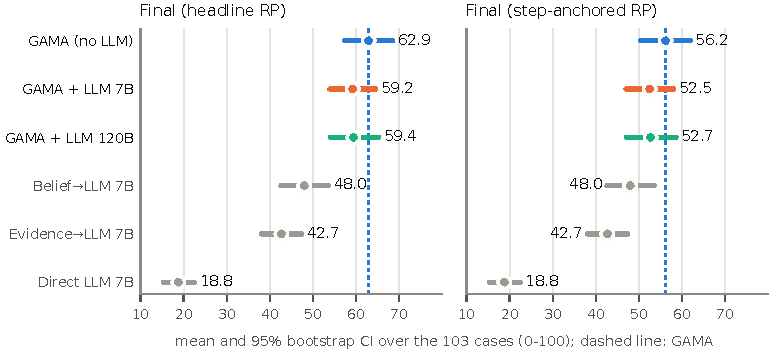
\includegraphics[width=\textwidth]{figs/fig2_main.pdf}
\caption{Final score of every arm on the 103 RCA100 cases with 95\% bootstrap intervals; left with the headline reasoning-process
score, right with the step-anchored one. The dashed line marks \core{}. Arms in which an LLM writes the chain return no evidence
items, so the retrieval-based half of the headline RP is zero for them; the step-anchored score compares chains on equal terms.}
\label{fig:main}
\end{figure}

\paragraph{By fault group}
\Cref{fig:groups} breaks EL and FI down by fault group. \core{} localises JVM-runtime faults perfectly and types 69\% of them;
resource and performance faults are typed in 80\% of the cases. Its weak spot is node faults (EL 22.3): a node fault slows every
service it hosts, and when the node's own CPU or memory signal does not stand out against its peers, a hosted service with strong
trace evidence wins. Middleware and database faults are localised (EL 77.9) but rarely typed (FI 23.1); plausibly because slow SQL and
database network latency look alike in spans when no database-side metrics are exported.

\begin{figure}[!htbp]
\centering
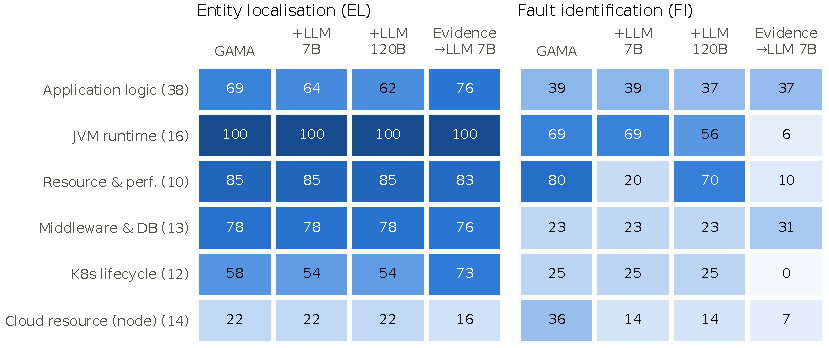
\includegraphics[width=\textwidth]{figs/fig3_groups.pdf}
\caption{Entity localisation (left) and fault identification (right) by RCA100 fault group, for \core{}, \core{} with the bounded LLM
(7B and 120B) and Evidence$\rightarrow$LLM (7B). Darker is better.}\label{fig:groups}
\end{figure}

\subsection{RQ2: contribution of the modules}\label{sec:ablation}

\Cref{tab:ablation} reports the leave-one-module-out runs. Removing trace-origin attribution (\Mod{2}) costs 5.6 Final points
[2.3, 9.3] ($p=0.009$; 18 cases better with the module, 5 worse): the module mainly identifies the \emph{type}
(exact type 14 : 2, McNemar $p=0.004$), because the messages and status codes of the origin spans name rate limiting, null pointers
and HTTP 5xx errors (application-logic FI 39.5 with the module versus 10.5 without). It costs node faults, however: node EL drops
from 33.9 to 22.3 with the module, since a node that hosts several origin services can lose to one of them, and a node without its
own signal can win on their strength. \pending{leave-one-out runs of \Mod{1}, \Mod{3}, \Mod{4}, \Mod{5} and \Mod{6}.}

\begin{table}[!htbp]
\centering
\caption{Leave-one-module-out ablation on the 103 RCA100 cases: change of the Final score when a module is removed from \core{}
(paired Wilcoxon, two-sided, Holm over the six modules), cases better / worse with the module, and McNemar counts for the exact
type (with : without).}\label{tab:ablation}
\footnotesize
\setlength{\tabcolsep}{4pt}
\begin{tabular}{@{}lcccc@{}}
\toprule
Module removed & $\Delta$Final [95\% CI] & $p$ & better / worse & exact type \\
\midrule
\Mod{1} corroboration & \tbd & \tbd & \tbd & \tbd \\
\Mod{2} trace origins & $-5.6$ [$-9.3$, $-2.3$] & 0.009$^\dagger$ & 18 / 5 & 14 : 2 \\
\Mod{3} mechanism typing & \tbd & \tbd & \tbd & \tbd \\
\Mod{4} load explain-away & \tbd & \tbd & \tbd & \tbd \\
\Mod{5} mechanism text & \tbd & \tbd & \tbd & \tbd \\
\Mod{6} cited chain (RP only) & \tbd & \tbd & \tbd & -- \\
\bottomrule
\end{tabular}
\begin{flushleft}\footnotesize $^\dagger$ unadjusted; the Holm adjustment is applied once all six runs are available.\end{flushleft}
\end{table}

\subsection{RQ3: what the language model adds}\label{sec:llmrole}

\paragraph{Decision}
With either backbone, the bounded LLM lowers the Final score of the statistical core (\cref{tab:llmtests}, \cref{fig:llm}a):
by 3.7 points with Qwen2.5-7B ($p=0.008$; 2 cases better, 14 worse) and by 3.5 points with gpt-oss-120b ($p=0.03$; 3 better, 13
worse). The two backbones end at the same score ($+0.2$, $p=0.62$). Two mechanisms are responsible (post-hoc analysis, no design
change). (i) \emph{Shortlist typing} changed the computed type in 25 (7B) and 21 (120B) cases; only 3 and 2 of these changes reached
the true type, while 10 and 7 replaced a correct type (\cref{fig:llm}b). The changes concentrate where the telemetry cannot separate
two types: the 7B model turned \emph{cpuFullLoad} into \emph{cpuDeadLoop} in seven cases; the 120B model avoided this pattern but
turned \emph{memoryPressure} into \emph{fullGC} in two; both models replaced node CPU faults by disk or memory faults (node FI 35.7
$\rightarrow$ 14.3). (ii) The \emph{text sensor} moved a correct entity away in four cases---the same four cases with both
backbones---which points to the weight of the sensor's answer in the likelihood rather than to the model.

\paragraph{The computed belief and a free LLM}
Given the posterior and full authority (Belief$\rightarrow$LLM), the 7B model kept \core{}'s entity and type in 102 of 103 cases
(the remaining case is a truncated answer that also repeated it): it defers to the computed belief (B1). The belief helps the LLM:
Belief$\rightarrow$LLM exceeds Evidence$\rightarrow$LLM by 5.3 points [0.2, 10.4] (one-sided $p=0.025$; exact type 33 : 9), confirming
B2. Compared with the bounded use of the same model (B3), the free LLM decides better (exact type 11 : 2), but its own chain is weaker
than the computed one (chain-node match 51.5 versus 72.7, step-anchored checkpoints 0.0 versus 0.307), so its Final$_\text{step}$ is
4.4 points lower.

\paragraph{Explanation}
Scale changes the explanation, not the decision (\cref{fig:llm}c). The narrator of gpt-oss-120b satisfies 0.284 of the step-anchored
evidence checkpoints against 0.107 for the 7B narrator on the same cases (51 cases higher, 5 lower; one-sided Wilcoxon
$p=2\times10^{-10}$), close to the computed chain (0.307); 88\% of the numbers it quotes appear in the evidence (7B: 92\%). This
supports H3.

\begin{figure}[!htbp]
\centering
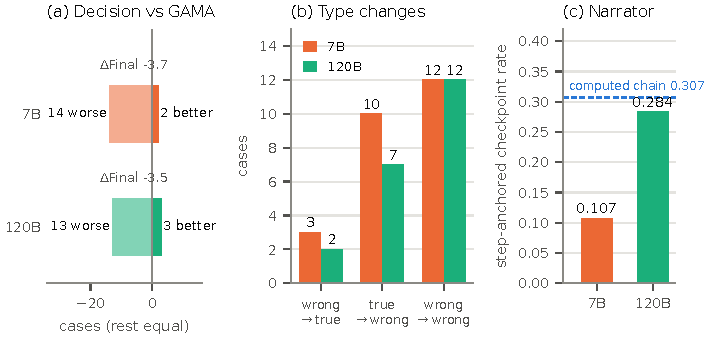
\includegraphics[width=\textwidth]{figs/fig4_llm.pdf}
\caption{What the bounded LLM adds. (a) Cases in which \core{} + LLM scores better or worse than \core{} (the remaining cases are
equal). (b) Changes of the computed type made by shortlist typing. (c) Step-anchored checkpoint rate of the LLM narrator; the dashed
line is the chain computed by \Mod{6}.}\label{fig:llm}
\end{figure}

\begin{table}[!htbp]
\centering
\caption{Pre-registered comparisons and hypotheses on the 103 RCA100 cases. $\Delta$ is the paired difference of Final scores
(first minus second) with 95\% bootstrap CI; $p$ from the Wilcoxon signed-rank test (Holm within family).}\label{tab:llmtests}
\footnotesize
\setlength{\tabcolsep}{3pt}
\begin{tabularx}{\textwidth}{@{}>{\raggedright\arraybackslash}X ccc>{\raggedright\arraybackslash}p{2.4cm}@{}}
\toprule
Comparison & $\Delta$Final [95\% CI] & $\Delta$Final$_\text{step}$ & $p$ & Outcome \\
\midrule
\core{} vs Evidence$\rightarrow$LLM (7B) & $+20.2$ [15.0, 25.6] & $+13.5$ & $2.8\times10^{-10}$ & structure wins \\
\core{}+LLM (7B) vs \core{} & $-3.7$ [$-6.4$, $-1.4$] & $-3.7$ & 0.008 & LLM lowers the score \\
\core{}+LLM (120B) vs \core{} & $-3.5$ [$-6.3$, $-0.9$] & $-3.5$ & 0.03 & LLM lowers the score \\
\core{}+LLM (120B) vs \core{}+LLM (7B) & $+0.2$ [$-2.2$, 2.6] & $+0.2$ & 0.62 & no effect of scale \\
\core{}+LLM (7B) vs Evidence$\rightarrow$LLM (7B) & $+16.5$ [11.8, 21.2] & $+9.8$ & $8.2\times10^{-10}$ & structure wins \\
B2: Belief$\rightarrow$LLM vs Evidence$\rightarrow$LLM (7B) & $+5.3$ [0.2, 10.4] & $+5.3$ & 0.025 & supported \\
B3: Belief$\rightarrow$LLM vs \core{}+LLM (7B) & $-11.2$ [$-13.8$, $-8.4$] & $-4.4$ & $1.6\times10^{-11}$ & better type, weaker chain \\
\midrule
H1: $|\Delta\text{EL}|\leq3$ & \multicolumn{3}{c}{7B: 2.4 \quad 120B: 3.2} & met for 7B, narrowly not for 120B \\
H2: FI gain $\leq$ shortlist coverage & \multicolumn{3}{c}{no FI gain with either backbone} & met \\
H3: narrator checkpoints rise with scale & \multicolumn{3}{c}{0.107 $\rightarrow$ 0.284, $p=2\times10^{-10}$} & supported \\
H4: \core{}+LLM (7B) $>$ Evidence$\rightarrow$LLM (120B) & \multicolumn{3}{c}{\pending{run}} & \\
H5: $\leq$ 7 LLM calls per incident & \multicolumn{3}{c}{mean 2.7, max 5 (both backbones)} & met \\
\bottomrule
\end{tabularx}
\end{table}

\subsection{Cost}\label{sec:cost}
\core{} needs no GPU and no model: 78\,s per incident on four CPU cores, most of it reading the incident's files. The bounded LLM
(\cref{tab:cost}) adds 2.7 calls and about 9,000 tokens per incident (7B: 181\,s on a T4; 120B: 128\,s through the API, where 1,200 of the 1,400 output
tokens are reasoning). The full 120B run of \core{}+LLM on 103 incidents cost about USD 0.40. For comparison, belief-state agents
consume about $1.8\times10^6$ tokens per RCA100 episode \citep{luo2026pos}, and open agents of the strongest configurations studied
by Lu et al.\ about $1.5\times10^6$ \citep{lu2026beyond}; their scores are not comparable with ours (different protocols and
backbones), but the two-to-three orders of magnitude in cost are.

\begin{table}[!htbp]
\centering
\caption{Cost per incident on RCA100 (means over 103 cases; time includes reading the incident's files).}\label{tab:cost}
\footnotesize
\begin{tabular}{@{}lcccc@{}}
\toprule
Arm & Hardware & s / case & LLM calls & tokens (input / output) \\
\midrule
\core{} (no LLM) & CPU, 4 cores & 78 & 0 & 0 \\
\core{}+LLM, 7B & T4 GPU & 181 & 2.7 & 9{,}157 (8{,}986 / 228) \\
\core{}+LLM, 120B & CPU + API & 128 & 2.7 & 9{,}012 (7{,}592 / 1{,}421) \\
Belief$\rightarrow$LLM, 7B & T4 GPU & 152 & 1 & 4{,}812 (4{,}585 / 227) \\
Evidence$\rightarrow$LLM, 7B & T4 GPU & 168 & 1 & 4{,}337 (4{,}128 / 209) \\
Direct LLM, 7B & T4 GPU & 38 & 1 & 983 (856 / 127) \\
\bottomrule
\end{tabular}
\end{table}

\subsection{RQ4: zero-shot transfer to AIOps2025}\label{sec:aiops}

\paragraph{Protocol}
The transfer was pre-registered before any run. What stays fixed is the method: the likelihood model, the roles, every constant, the
decision and the modules. What may change is dataset knowledge written without AIOps2025 labels: (A1) an adapter from the release
files to the canonical incident; (A2) metric-name patterns (e.g.\ \texttt{rrt} $\rightarrow$ latency) and the failing-span status;
(A3) a topology derived from parent--child spans and from the published architecture (AIOps2025 ships no topology); (A4) pod
entities with one rule---a service-level fault shows its mechanism in every pod, a pod-level fault in one pod while its siblings
stay normal; (A5) fingerprints for the AIOps2025 fault types written from their published definitions; (A6) the benchmark's output
format; (A7) trace sampling (all failing traces and a fixed hash-selected 20\% of the others). A synthetic release in the real file
layout tests the adapter (a CPU fault in one pod is located at that pod, in all pods at the service) and that ground-truth files are
never opened. An implementation audit before the run found that the planned removal of other incidents' windows from the history
would leave too little history for the frozen coverage rule (\cref{eq:shift}); it was replaced, before any run, by the robust
history statistics already in the method.

\paragraph{Results}
\pending{AIOps2025: label-free checks (adapter coverage, testable and holding signals), then one run on the 400 cases; LA, TA,
explainability, efficiency and the benchmark Final score with bootstrap CIs; breakdown by fault category and level (service / pod /
node). Context, not a controlled comparison: the published accuracy of LLM agents on AIOps2025 \citep{lu2026beyond}.}

\section{Discussion}\label{sec:discussion}

\paragraph{Why a computed belief}
The comparison of Evidence$\rightarrow$LLM, Belief$\rightarrow$LLM and \core{} separates three ingredients: good evidence, a belief
over hypotheses, and who decides. Calibrated evidence alone lets a 7B model localise as well as the statistical core, but not type
the fault (FI 20.4 versus 43.7): choosing among 28 types requires weighing many weak signals against each other and against their
background rates, which a likelihood does consistently and a language model does not. Once the posterior is given, the same model
adopts it almost always. The belief is therefore the part that carries the diagnosis, and it can be computed. This complements
belief-state agents \citep{luo2026pos,luo2026graphofstates}: their beliefs are written by the model at a cost of millions of tokens,
ours is computed from calibrated likelihoods in seconds, and an LLM can still read it.

\paragraph{Where an LLM helps}
Bounding the LLM did not make it a better decision maker: when the evidence does not separate two types, the model chooses the more
specific one and loses more often than it wins, at 7B and at 120B alike. Scale changes the narrative instead---the larger model's
chain cites the right values at the right steps almost as often as the computed chain. The practical design that follows is a
separation of duties: the decision and its evidence are computed and auditable, and the language model explains them. The results
also suggest how a later version could let an LLM contribute to the decision without the damage observed here: as a sensor whose
answers are calibrated like any other categorical observation (against the incident's own background rate), or as a typing step
that must defer to the posterior unless it quotes evidence that discriminates between the top types. Because these ideas were
formed after seeing the RCA100 results, they must be evaluated on data not used for their design.

\paragraph{Failure modes ruled out by construction}
Several reasoning failures that Lu et al.\ \citep{lu2026beyond} observe in LLM agents cannot occur in \gama{} by construction
(\cref{tab:failuremodes}): every signal is tested against a baseline, every entity's resource signals are computed, timing enters as
onset precedence, caller and callee roles are fixed by the trace structure and the load direction, and the whole hypothesis space is
scored at once rather than anchored on the first idea. The remaining errors are mostly limits of the evidence---node faults without a
distinctive node signal, database faults without database metrics---rather than of the reasoning.

\paragraph{Threats to validity}
\emph{Internal.} RCA100 was the development data; although each change was pre-registered and the final modules were developed on
half of the cases, the 103-case results are optimistic, and we make no held-out claim on them. The fingerprint tables were written
from the published fault definitions, but their additions were informed by development errors. \emph{Construct.} Our scorer
re-implements the published RCA100 protocol; the retrieval-based half of the headline RP is independent of the decision and
favours systems that return evidence items, which is why every comparison is also reported with the step-anchored variant. The
Final weights of the benchmark (0.4 / 0.3 / 0.3) are taken as given. \emph{Statistical.} With 103 cases, differences of about three
points are at the edge of detectability; we report intervals and exact case counts with every test. API decoding is not
deterministic; we report the single pre-registered run of each arm. \emph{External.} RCA100 covers one application on one platform;
the AIOps2025 transfer (\cref{sec:aiops}) tests a second system with different fault types and pod-level faults. Two backbones do not
span the space of LLMs; a stronger reasoning model or a different interface may behave differently.

\paragraph{Ethics and data}
No personal data are involved. Both benchmarks are used under their non-commercial licences and are not redistributed. The API runs
used a provider setting without data retention; prompts contain only benchmark telemetry.

\section{Conclusion}\label{sec:conclusion}

\gama{} computes the diagnosis of a microservice incident: calibrated multimodal evidence updates a Bayesian belief over (entity,
fault type) hypotheses that explains symptoms away along the topology, estimates its propagation strength per incident and respects
temporal precedence; a two-stage decision and an evidence-cited chain follow. Without labels, training or a language model, it
reaches 62.9 Final on the 103 RCA100 cases on a CPU, 20.2 points above a 7B LLM that decides from the same evidence. In a
pre-registered study, a bounded LLM did not improve the decision at 7B or at 120B parameters, while the larger model wrote a far
better explanation. The decision should be computed and the language model should explain it. Future work covers the zero-shot
AIOps2025 evaluation (\cref{sec:aiops}), node faults without distinctive node signals, and LLM roles that enter the belief only as
calibrated evidence, evaluated on data not used for their design.


\section*{CRediT authorship contribution statement}
\pending{roles of each author (Conceptualization, Methodology, Software, Validation, Writing -- original draft, \ldots).}

\section*{Declaration of competing interest}
The authors declare that they have no known competing financial interests or personal relationships that could have appeared to
influence the work reported in this paper.

\section*{Data and code availability}
The code (the \texttt{gama/} package, the evaluation scripts, the pre-registration documents and the synthetic tests) is available
at \url{https://github.com/solaemanachmad/gamarca}. Every run writes a manifest (commit, modules, model, hardware, library versions,
wall time), the scored results, the decision trail of every case and every LLM call (prompt, output, input and output tokens,
latency); these artefacts are released with the code. RCA100 (CC BY-NC-SA) and AIOps2025 (CC BY-NC 4.0) are obtained from their
publishers and are not redistributed.

\section*{Declaration of generative AI and AI-assisted technologies in the writing process}
\pending{Elsevier declaration: state which AI-assisted tools were used, for which tasks (e.g.\ code development, language editing),
and that the authors reviewed and edited the content and take full responsibility for it.}

\section*{Acknowledgements}
This research was supported by the Hibah DAMAS Penelitian 2026 of Sekolah Vokasi, Universitas Gadjah Mada.

\appendix
\section{Constants}\label{app:constants}

\begin{table}[H]
\centering
\caption{Constants of \gama{}, fixed a priori (none fitted to labels).}\label{tab:constants}
\footnotesize
\setlength{\tabcolsep}{4pt}
\begin{tabularx}{\textwidth}{@{}>{\raggedright\arraybackslash}p{2.6cm} >{\raggedright\arraybackslash}p{2.7cm} >{\raggedright\arraybackslash}X@{}}
\toprule
Symbol & Value & Meaning \\
\midrule
$\alpha$ & 0.05 & level at which a calibrated signal holds; background of a continuous observation \\
$B$, $K$ & 4, 5 & history length (window lengths) and number of pseudo-windows \\
coverage & 0.8 / 0.5 & minimum sample coverage of the history / the window \\
scale floors & $0.05|\median|$, 1 & relative floor of the robust scale; floor of own-volatility and peer re-standardisation \\
peers, pool & $\geq3$, $\geq20$ & minimum peers; minimum null pool (else pooled over the entity kind) \\
onset & 3 SD, 2 samples & onset threshold of a holding signal \\
$\theta_K$ & 0.8 & probability that some key signal holds at the true root \\
$\theta_U$ & 0.6 & support / may signal at the root \\
$\theta_P$ & 0.6 & own symptom at the root; load explained from upstream \\
$\alpha_C$ & 0.05 & contradicting signal at the root \\
categorical background & Beta, 10 pseudo-entities & shrinkage of the per-incident share towards $\alpha$ \\
$\Pr(h_0)$, fallback weight & 0.1, 0.5 & prior of no fault; prior weight of the two fallback types \\
$\pi$ & $[0.06,0.95]$, 30 iterations & EM bounds and iteration limit for the propagation strength \\
$\theta_T$, tolerance & 0.9, 60\,s & temporal precedence (onsets and intra-entity order) \\
$\theta_M$, $\beta_M$ floor, weight & 0.6, 0.1, 10 & cross-modal corroboration (\Mod{1}) \\
trace origins & 30\%, 10 / 5 traces & error origin share and minimum error / slow traces (\Mod{2}) \\
chain & 4 values per step & window values cited per chain step (\Mod{6}) \\
sensor & $\Pr\geq0.8$, 0.05 bits, 5 probes & stop rule, minimum information gain, budget (\Mod{7}) \\
typing & top 5, quote $\geq10$ chars & shortlist size and quote length (\Mod{7}) \\
decoding & temp.\ 0, seed 0 & greedy decoding; 1,024 new tokens (local), 8,192 incl.\ reasoning (API) \\
\bottomrule
\end{tabularx}
\end{table}

\section{Fingerprint examples}\label{app:fingerprints}

\begin{table}[H]
\centering
\caption{Excerpt of the RCA100 fingerprint table (roles of signals per fault type; ``a\&b'' requires both). The full table and the
AIOps2025 table are in the code.}\label{tab:fingerprints}
\footnotesize
\begin{tabularx}{\textwidth}{@{}l>{\raggedright\arraybackslash}X>{\raggedright\arraybackslash}X>{\raggedright\arraybackslash}X@{}}
\toprule
Type & Key (one of) & Support & Contradiction \\
\midrule
nodeCpuHigh & node CPU rise & -- & -- \\
nodeDown & node NotReady event; node ready drop & node pods drop & scale-down event \\
cpuFullLoad & CPU rise & latency rise & request rise \\
memoryPressure & memory rise & GC rise, CPU rise & -- \\
fullGC & GC rise & GC log rise, GC message, latency rise & -- \\
rateLimiting & HTTP 429; rate-limit message or log rise & HTTP 403 & -- \\
trafficSurge & request rise & latency rise, CPU rise & -- \\
replicaScaleDown & scale-down event; replica / availability drop; unavailable & HTTP 503, connection refused, request drop & crash-loop, unschedulable \\
redisUnavailable & failing Redis spans; Redis message & connection refused, timeout & -- \\
slowSQL & slow database spans & latency rise, SQL message & failing database spans \\
httpError5xx (fallback) & HTTP 5xx & failing spans, error rise & -- \\
\bottomrule
\end{tabularx}
\end{table}

\section{Agent failure modes ruled out by construction}\label{app:failuremodes}

\begin{table}[H]
\centering
\caption{Failure modes of LLM agents catalogued by Lu et al.\ \citep{lu2026beyond} and the mechanism of \gama{} that prevents each.}
\label{tab:failuremodes}
\footnotesize
\begin{tabularx}{\textwidth}{@{}>{\raggedright\arraybackslash}p{4.3cm}>{\raggedright\arraybackslash}X@{}}
\toprule
Failure mode & Mechanism in \gama{} \\
\midrule
Baseline gap (no comparison with normal behaviour) & every signal is scored against the incident's own history (stage 1) \\
Edge untested & propagation is explained only along topology edges; trace origins test caller--callee spans (\Mod{2}) \\
Resource gap & the resource signals of every entity are always computed; there is no query choice \\
Ranking gap & peer re-standardisation rejects shifts common to all entities of a kind \\
Timing gap & onset precedence (stage 2) and intra-entity signal order (\Mod{3}) \\
Silence taken as health & availability and replica drops are observations \\
Salience bias (chronically noisy entity) & own-volatility re-standardisation; EM penalises wide hypotheses \\
Caller / callee semantics reversed & trace origin with callee relay (\Mod{2}); directional load explain-away (\Mod{4}) \\
Anchor lock & no sequential anchoring: all hypotheses are scored at once \\
Schema-out claim (type outside the taxonomy) & typed hypothesis space; the LLM chooses only within the shortlist (\Mod{7}) \\
Friction stop & fixed pipeline without a tool loop \\
\bottomrule
\end{tabularx}
\end{table}


\bibliographystyle{elsarticle-num}
\bibliography{refs}

\end{document}
